\documentclass[byrevtex,amssymb,aps,pra,floatfix,letterpaper]{revtex4}
\usepackage{graphicx}
\usepackage{hyperref}
\usepackage{amsmath}
\bibliographystyle{apsrev}
\date{\today}
\pagestyle{plain}
\newcommand{\degree}[0]{$^\circ$}

\begin{document}

\title{Experiment 1: Adiabatic Bomb Calorimeter}

\date{\today}

\maketitle

\section{Introduction}

Heat released in a chemical reaction can be determined experimentally by using an adiabatic calorimeter. The reaction must proceed without any side reactions and sufficiently fast that the heat exchange with the surroundings is  negligible. The heat of combustion can be most conveniently measured using an  adiabatic bomb calorimeter. In such calorimeter, the combustion reaction  occurs in a closed container under constant volume (``bomb''). The bomb is immersed in a weighted quantity of water and surrounded by an adiabatic shield that serves as a heat insulator. Continuous stirring ensures that heat is distributed evenly in the calorimeter. The bomb and the water bath, which are in direct thermal contact, constitute an adiabatic bomb calorimeter. In this experiment the heat of combustion of an organic compound is determined using a commercial Parr adiabatic bomb calorimeter. The heat of combustion is directly related to important quantities such as the internal energy and enthalpy of a chemical reaction. A more detailed overview of the thermodynamic approach can be found from Refs. \cite{ATKINS1,SILBEY,CHANG}.

\section{Theory}

\subsection{Internal energy of combustion}

According to the first law of thermodynamics, a change in internal energy  depends on heat transfer between the system and the surroundings ($q_{syst} < 0$ and $q_{surr} > 0$) and work done by/on the system ($w$):

\begin{equation}
\label{eq1}
\Delta U = q_{syst} + w
\end{equation}

\noindent
Recall that both $q$ and $w$ indicate changes in properties even though we have not written $\Delta$ in front of them. If we assume that only pressure ($P_{ext}$) - volume ($V$) work is done and the volume is constant (i.e., $\Delta V = 0$), we have:

\begin{equation}
\label{eq2}
w = -P_{ext}\Delta V = 0
\end{equation}

\noindent
Note that $P_{ext}$ denotes the external pressure against which the system does work. If the process is reversible, the internal pressure ($P$) and $P_{ext}$ are identical. The first law at constant volume now becomes:

\begin{equation}
\label{eq3}
\Delta U = q_{syst}
\end{equation}

\noindent
In an adiabatic bomb calorimetric experiment, changes in the water bath temperature ($\Delta T$) are measured. If the heat capacity $C_{cal}$ of the 
calorimeter (surroundings) is known, the amount of the heat released by the bomb (i.e., chemical combustion reaction) is given by:

\begin{equation}
\label{eq4}
-q_{syst} = q_{surr} = C_{cal}\Delta T_{surr}
\end{equation}

\noindent
Thus $\Delta U$ is the quantity that an adiabatic bomb calorimeter determines directly through the measurement of $q_{surr}$.

\subsection{Enthalpy of combustion}

The enhalpy ($H$), which in the present case is enthalpy of combustion, is defined as:

\begin{equation}
\label{eq5}
H = U + PV
\end{equation}

\noindent
and correspondingly a change in $H$ (denoted by $\Delta H$) is given by:

\begin{equation}
\label{eq6}
\Delta H = \Delta U + \Delta (PV) = \Delta U + \underbrace{P\Delta V}_{= 0}
+ V\Delta P = \Delta U + \underbrace{V\Delta P}_{\ne 0} \ne \Delta U
\end{equation}

From the above expression, we see that $\Delta U$ and $\Delta H$ would be identical only if the pressure in the bomb remains constant. If the amount of gases in the bomb remain constant, $\Delta P$ would be zero and thus $\Delta U = \Delta H$. However, in most combustion reactions the molar amounts of gases change and therefore a method for calculating the $\Delta(PV)$ term in Eq. \ref{eq6} is required. If we assume that the gaseous components in the bomb behave according to the ideal gas law ($PV = n_{gas}RT$), we can write:

\begin{equation}
\label{eq7}
\Delta (PV) = R\Delta (n_{gas}T) = RT\Delta n_{gas} + 
\underbrace{Rn_{gas}\Delta T}_{\textnormal{``small''}} \approx RT\Delta n_{gas}
\end{equation}

\noindent
where $R$ is the gas constant (8.31 J mol$^{-1}$ K$^{-1}$). The term denoted by ``small'' can be neglected when changes in temperature are small (couple of \degree C). Note that $\Delta n_{gas}$ can be either positive (the amount of gaseous components increase) or negative (the amount of gaseous components decrease). 
Also the contribution of liquids and solids to the $\Delta PV$) -- term is negligible.\\

\noindent
\textbf{Example.} The combustion reaction of benzoic acid at 25 \degree C is:

\begin{equation}
\label{eq8}
\textnormal{C}_6\textnormal{H}_5\textnormal{COOH(s)} + \underline{7.5}
\textnormal{O}_2\textnormal{(g)} \rightarrow\underline{7}\textnormal{CO}_2
\textnormal{(g)} + 3\textnormal{H}_2\textnormal{O(l)}
\end{equation}

\noindent
In this case, for one mole of $\textnormal{C}_6\textnormal{H}_5\textnormal{COOH(s)}$, $\Delta n_{gas} = 7 - 7.5 = -0.5$ mol. Hence for the combustion of one mole of benzoic acid we have:

\begin{equation}
\label{eq9}
\Delta H = \Delta U + \left( -\frac{1}{2} \textnormal{ mol}\right)
\times \left( 8.31 \frac{\textnormal{ J}}{\textnormal{ mol K}}\right)
\times \left( 298 \textnormal{ K}\right) = \Delta U - 1240 \textnormal{ J}
\end{equation}

\section{Apparatus and chemicals}

A commercial bomb calorimeter (Parr) is a self-contained instrument used in determination of heats of combustion of certain fuels and pure organic substances. The results obtained are sufficiently precise to make them of extreme importance in most commercial and laboratory procedures concerned with heats of combustion.

The combustion bomb, made of corrosion-resistant metal, holds the sample whose heat of combustion is to be measured. The sample is held in a cup as shown in Fig. \ref{fig1}. Fig. \ref{fig2} shows how the ignition wire, used to start the combustion reaction, is attached to the electrodes. After the sample and the wire have been properly placed in the bomb, it is charged with oxygen gas from a commercial cylinder to the pressure of about 25 atm.

\begin{figure}[!htp]
\begin{center}
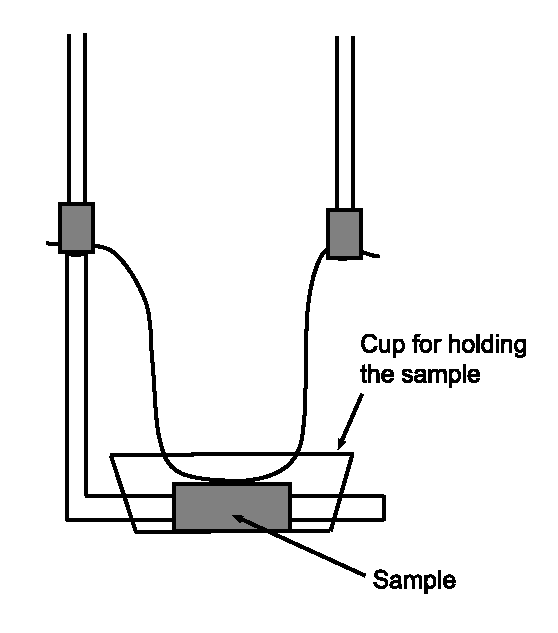
\includegraphics[scale=0.5]{calorimeter}
\caption{Schematic of the sample support stand. Note positioning of the ignition wire (about 1 mm from the sample but not touching it).}
\label{fig1}
\end{center}
\end{figure}

\begin{figure}[!htp]
\begin{center}
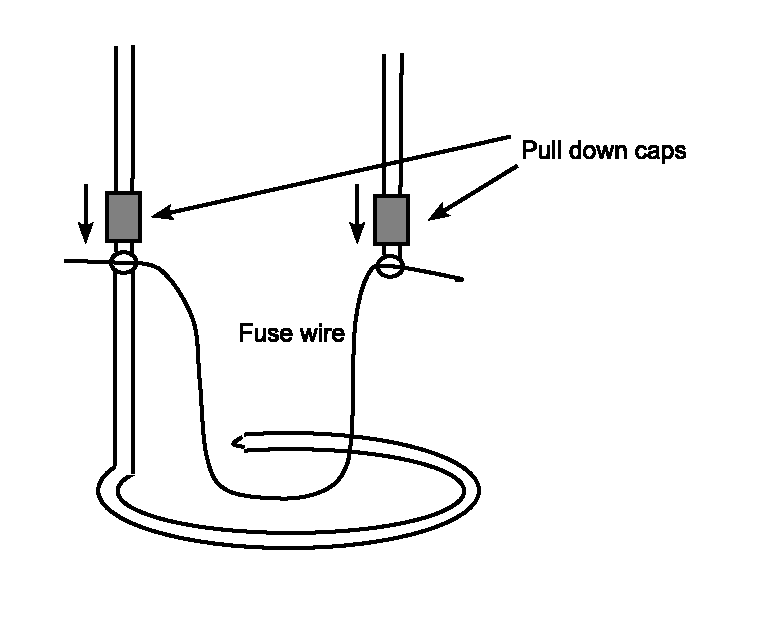
\includegraphics[scale=0.5]{wire}
\caption{Attachment of the nichrome ignition wire. The caps on the electrodes fix the ignition wire.}
\label{fig2}
\end{center}
\end{figure}

The assembled bomb is then placed in a bucket containing a specified quantity of water. The temperature rise accompanying the combustion is read from a thermometer. A stirrer effects an even distribution of the water. The bucket in turn is surrounded by an insulating air space, which prevents, as far as possible, heat leakage to the surroundings.

First, it is necessary to obtain the heat capacity of the calorimeter system ($C_{cal}$). This is the number of calories necessary to raise the temperature of the entire calorimeter system by one degree centigrade. This is found by burning a sample material of known heat of combustion. Benzoic acid of high purity is usually employed. The temperature rise due to the sample is noted, and the number of joules of heat released in the combustion is calculated. These two values enable one to calculate the heat capacity of the calorimeter system. This is then used to calculate the heat of combustion of the assigned material.\\

\noindent
\underline{Required materials:} (I) Parr calorimeter system including firing mechanism, stirrer, etc., (II) pellet press, (III) two digital thermometers with 0.01 \degree C accuracy, (IV) ignition wire, (V) oxygen cylinder, (VI) benzoic acid, and (V) unknown sample (naphthalene).

\section{Sample preparation and measurement}

\noindent
\underline{Task overview:} Carry out at least three independent measurements of the benzoic acid standard and at least three independent measurements of the ``unknown'' sample (i.e., naphthalene).\\

\noindent
\underline{Pellet preparation:} Care must be taken to avoid overcharging the bomb for it must be realized that the peak pressure developed during combustion is proportional to the size of the sample and to the initial oxygen pressure. Pellet size should be limited to not more than 1.1 g. Prepare the pellet:\\

\noindent
1. Weigh out approximately 1.0 g of sample. Grind it in a clean mortar and pestel.\\
2. Use the pellet press to make a pellet and weigh it.\\
3. Carefully place it in the sample cup with tweezers. Do not touch it with your hands!\\

\noindent
\underline{Connect the ignition wire:}\\

\noindent
\begin{enumerate}
\item Measure out approximately 10 -- 11 cm of wire and weigh it. It will also be necessary to weigh any unburned wire after combustion since this is an important factor in the calculations.

\item Set the bomb head in the support stand and attach the length of nichrome fuse wire as illustrated in Fig. \ref{fig2}. A pair of tweezers may be helpful in attaching the wire to the electrodes. Insert the wire through each eyelet then slide each cap downward to complete the connection.

\item Place the sample cup (with the sample sitting in the center of the cup) in the cup holder and bend the nichrome wire in a V-shape. Position the wire so that it almost touches the surface of the pellet (about 1 mm separation). Fig. \ref{fig1} illustrates the proper installation and sample placement. Make sure that the wire does not touch the cup.
\end{enumerate}

\noindent
\underline{Liquids in the bomb:} Pipet 1.0 mL of deionized water into the bomb to absorb the oxides of nitrogen formed from nitrogen present in the oxygen mixture.\\

\noindent
\underline{Close the bomb assembly:}\\

\noindent
\begin{enumerate}

\item Care must be taken not to disturb the sample when sealing and charging the bomb. Slide the head assembly into the bomb cylinder, screw open the vent cap on the head assembly to allow air to be expelled, and push the head down as far into the cylinder as it will go.

\item Close the vent cap tightly. A tight seal is required to prevent oxygen leaks.

\item Check the circuit with an ohmmeter. If the resistance is too large ($>>$ 100 $\Omega$), open the bomb and check the wiring.

\end{enumerate}

\underline{Install the oxygen connection:}\\

\begin{enumerate}

\item Carefully secure the bomb in the bench clamp.

\item Slip on the oxygen tank connection hose to the pin on the head assembly.

\end{enumerate}

\underline{Fill the bomb:}\\

\begin{enumerate}
\item Open the oxygen tank valve. Open the regulator valve slowly and watch the gauge as the bomb pressure rises to the desired filling pressure (25 -- 30 atm). Once this pressure is reached close the control valve and then the tank valve. Note: If the bomb is filled too quickly you can blow your sample out of the sample cup. Warning: Do not exceed the specified pressure!

\item Use the quick-release valve to quickly remove the oxygen tank connection to minimize oxygen escape. Slight leakage is normal but continuous leakage is a problem.

\end{enumerate}

Possible problems:

\begin{enumerate}

\item If there is a continuous escape of gas from the bomb head connections once the oxygen tank valve is unscrewed the bomb is defective and should not be used.

\item If the bomb will not hold pressure and you can hear oxygen escaping around the vent cap, then the cap is not sealed tightly enough. Tighten down the screw cap by hand again and try to pressurize the bomb. If you are not successful after one or two attempts use a new bomb -- do not fire a leaking bomb!

\item If too much oxygen should accidentally be introduced into the bomb, do not proceed. Unscrew the oxygen tank connection and exhaust the bomb in the hood. This can be done by opening the vent cap. Reweigh the sample before repeating the filling procedure.

\end{enumerate}

\underline{Operating the calorimeter:}\\

\begin{enumerate}

\item Remove the lid and place it on the ring stand. Check to see that the bucket is resting properly in the jacket, noting the four pegs on the bottom of the jacket, which hold the bucket in place.

\item Carefully place the charged bomb in the bucket, noting that it rests on the raised circular area on the bottom of the bucket.

\item Connect the ignition wire to the terminal socket on the bomb head. Fill the bucket with the 2 L of water. Make sure that the digital thermometer can measure the initial water temperature. A typical temperature increase during the experiment will be around $<$ 4 $^{\circ}$C.

\item Set the cover on the jacket. The screw attached to the lid fits into the screw hole in the ledge of the jacket.

\item Turn the stirrer by hand to be sure that it runs freely, then slip the drive belt onto the pulley. If the belt does not work properly, rubber bands can be used.

\item Insert the thermometer sensor probe through the calorimeter top so that the end of the sensor touches the water.

\item Connect the two lead wires on the ignition unit to the calorimeter. Do not press the firing button unless the lead wire inside the jacket is connected to a bomb.

\item Plug in the calorimeter, ignition unit (use the 10 cm connector and ground) and timer. If the stirrer does not turn automatically check to see that it is turned on.

\item Let the stirrer run for 5 min to reach equilibrium. At the end of this period start the timer, and read and record the temperature at one-minute intervals for 5 min. At the start of the sixth minute stand back and fire the bomb by pressing the ignition button and holding it down for about 5 s (until the light goes out). \textbf{Caution: Don't have any parts of the body over the calorimeter when firing the bomb. Continue to stand clear for 30 s.}

\item The temperature should start to rise within 20 s of firing. Take the first temperature reading at 30 s and continue to take temperature readings every 15 s for a period of 2 min. The temperature should be read to the nearest 0.02 $^{\circ}$C. The reading lens is not required at this point.

\item After this two-minute period record the temperature to the nearest tenth (\textit{ca.} 0.002 $^{\circ}$C accuracy) with the aid of the reading lens at one-minute intervals until the difference between successive readings is zero (or perhaps becomes negative). This will take approximately five minutes. Accurate time and temperature observations must be recorded to identify certain points needed to calculate the calorific value of the sample. Usually the temperature will reach a maximum and then drops very slowly. Possible problems:

\begin{enumerate}

\item No significant temperature rise (1 $^{\circ}$C within 1 min). Check to see that the ignition unit is plugged in and all electrical connections are tight. Ignite the bomb again.

\item If this does not solve the problem it will be necessary to turn off all electrical connections, discharge the bomb in the hood and open it up. Place the bomb in the hood and open the valve to release the pressure. If the pellet is still intact but fuse wire is partially burned re-wire the bomb, weigh the pellet again, charge the bomb and ignite it again. If the pellet is only partially burned start over.

\end{enumerate}

\item After the last temperature reading, turn off all the electrical connections, remove the drive belt, and place the cover in support ring. Remove the ignition wire from the bomb, lift the bomb out of the bucket and wipe off any excess water. Open the valve cap and discharge the bomb in the hood. Unscrew the cap, lift the head out of the cylinder, and place it on the support stand.

\item Weigh any unburned fuse wire still attached to the electrodes and possible pieces of molten wire. When analyzing your results, you will need to subtract this weight from the total fuse wire burned. Examine the interior of the bomb for soot or other evidence of incomplete combustion. If such evidence is found the test will have to be discarded.

\end{enumerate}

\section{Utilization of data}

\noindent
\underline{Plotting the data:}\\

\noindent
Plot the (temperature, time) data for each run as illustrated in Fig. \ref{fig3}. Note the important points in the graph denoted by 'i', 'a', 'b', 'c', and 'f'. The point '$a$' denotes the time of firing of the bomb, '$b$' the position where the temperature reaches 60 \% of the total change, and '$c$' the time of maximum temperature (i.e., end of the reaction). Points '$i$' and '$f$' denote the initial and final points of measurement, respectively. The accuracy for reading the points should be to nearest 0.1 min. A simple approach for obtaining the temperature rise would consist of subtracting the initial and final temperatures (i.e., $\Delta T = T_c - T_a$). However, if the temperature is not stable in the initial ($i < t < a$) and final ($f > t > c$) periods, baseline correction must be applied. If the baseline is assumed to be linear, the rates of change can be obtained by using a difference approximation:

\begin{figure}[!htp]
\begin{center}
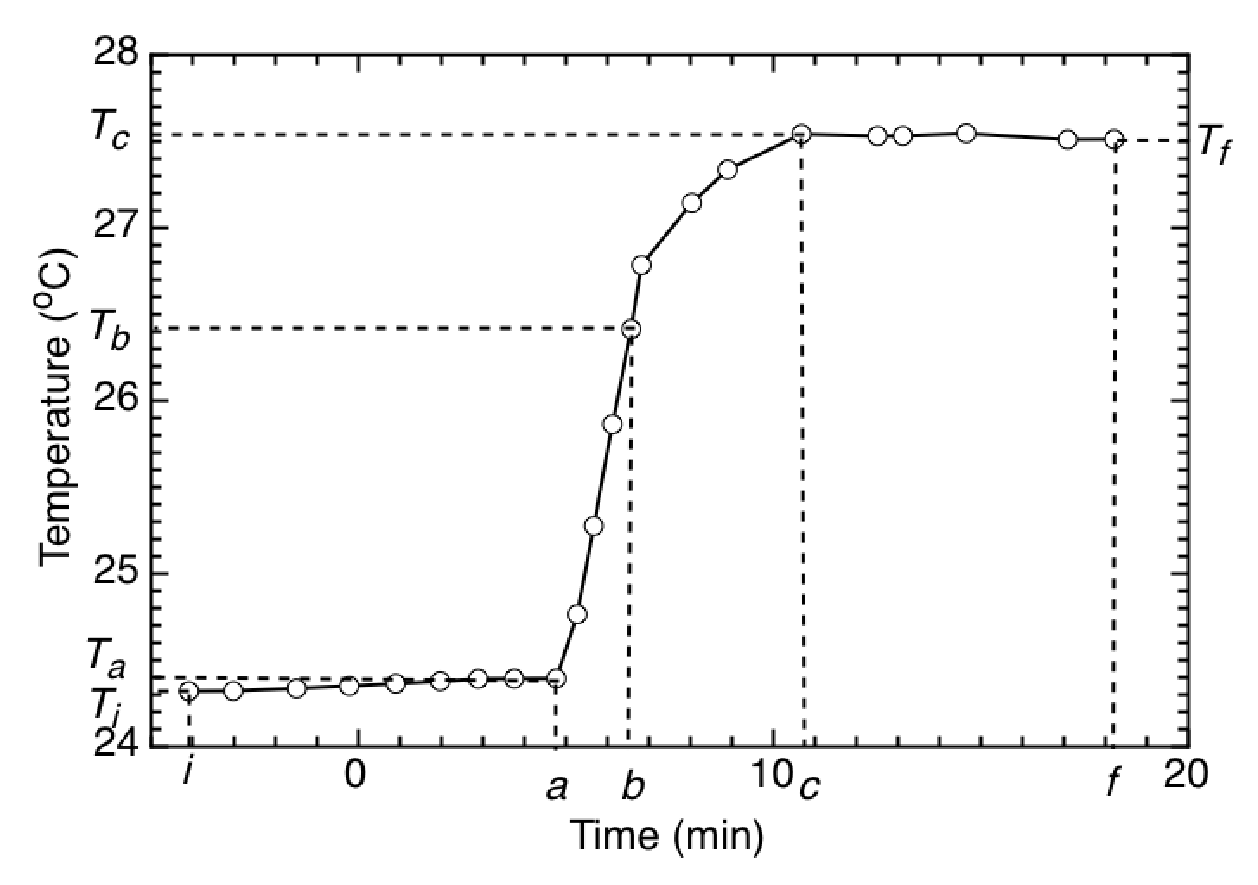
\includegraphics[scale=0.4]{graph}
\caption{An example of (temperature, time) data plot showing the positions for reading $T_i$, $T_a$, $T_b$, $T_c$, and $T_f$. For definitions of points '$i$', '$a$', '$b$', '$c$', and '$f$' see the text.}
\label{fig3}
\end{center}
\end{figure}

\begin{equation}
\label{eq10}
r_1 \approx \frac{T_a - T_i}{a - i}\textnormal{ and } r_2 \approx = \frac{T_f - T_c}{f - c}
\end{equation}

\noindent
The baseline is evaluated for both initial and final temperatures about point $b$:

\begin{equation}
\label{eq11}
\Delta T = \left(T_c - r_2(c - b)\right) - \left(T_a - r_1(b - a)\right) = T_c - T_a - r_1(a - b) - r_2(c - b)
\end{equation}

\noindent
This is the expression for the baseline corrected temperature rise.\\

\noindent
\underline{Heat capacity of the calorimeter}\\

\noindent
Before Eq. (\ref{eq4}) can be applied to find $q_{sys}$ (and $\Delta U$), $C_{cal}$ must be determined. In this experiment a specified amount of benzoic acid will be used as a standard. By measuring the $\Delta T$ (see Eq. (\ref{eq10})) using this standard, the heat capacity of the calorimeter can be calculated as follows:

\begin{equation}
\label{eq12}
C_{cal} = \frac{nq_{\tiny std,surr} + m_{\tiny wire}q_{\tiny wire,surr}}{\Delta T}
\end{equation}

\noindent
where $n$ is the amount of benzoic acid in the pellet (mol), $q_{\tiny std,surr}$ is the known heat of combustion of benzoic acid that is released to the surroundings (the literature value \cite{ATKINS1} is: $q_{\tiny std,surr} = -q_{\tiny std,sys} = -(\Delta H - RT\Delta n_{\tiny gas})$ = (3226.9 $-$ 1.2) kJ mol$^{-1}$ = 3225.7 kJ mol$^{-1}$ at 25 $^{\circ}$C; ``the molar enthalpy -- the $\Delta (PV)$ correction''), $m_{\tiny wire}$ (g) is the amount of the fuse wire used in the experiment, and $q_{\tiny wire,surr}$ is the heat of combustion per one gram of fuse wire (5.858 kJ g$^{-1}$; type Parr 45C10 nickel chromium fuse wire). Note that here $C_{\tiny cal}$ is a positive quantity.\\

\noindent
\underline{Heat of combustion of the sample}\\

\noindent
After determining $C_{\tiny cal}$, one can use this value (average of the runs) to calculate the gross heat of combustion (J mol$^{-1}$) of the sample in question:

\begin{equation}
\label{eq13}
\Delta \overline{U} = \overline{q}_{\tiny sys} = -\left( \mathop{\underbrace{\overline{q}_{\tiny surr}}}\limits_\textnormal{\tiny sample + wire} - \overline{q}_\textnormal{\tiny wire,surr}\right) = -\frac{C_{\tiny cal}\Delta T - m_{\tiny wire}q_{\tiny wire,surr}}{n}
\end{equation}

\noindent
where the over bars highlight that we are dealing with molar quantities and n denotes the molar amount of the substance. Note that Eq. (\ref{eq12}) is essentially identical to Eq. (\ref{eq4}) with the exception that it is written in terms of molar quantities and it includes the fuse wire correction. The fuse wire used for igniting the sample is partly consumed in the combustion. Thus the fuse generates heat both by the resistance it offers to the electrical current and by the heat of combustion of that portion of the wire, which is burned. The heat generated by the resistance is constant and small and thus can be neglected. However, the amount of wire consumed will vary from test to test and therefore a correction must be made to account for the heat of combustion of the metal.\\

\noindent
\underline{Enthalpy of combustion}\\

\noindent
According to Eqs. (\ref{eq5}) and (\ref{eq6}), the enthalpy of combustion is related to the heat of combustion by the follow relation:

\begin{equation}
\label{eq14}
\Delta \overline{H} \approx \Delta \overline{U} + RT\Delta n_{\tiny gas}
\end{equation}

\noindent
where the overbar again indicate molar quantities. Recall that both $\Delta H$ and $\Delta U$ here are negative because the system is releasing heat during combustion. The combustion reaction for naphthalene is:

\begin{equation}
\label{eq15}
\textnormal{C}_{10}\textnormal{H}_8(\textnormal{s}) + 12\textnormal{O}_2(\textnormal{g}) \rightarrow 10\textnormal{CO}_2(\textnormal{g}) + 4\textnormal{H}_2\textnormal{O}(\textnormal{l})
\end{equation}

\noindent
From this equation, we can see that $\Delta n_{\tiny gas} = -2$ for one mole of substance.

\section{Error analysis}
\label{sec6}

In this case, a simple error analysis is sufficient. Estimate the error in $C_{\tiny cal}$, $\Delta U$ and $\Delta H$ by calculating the standard deviation of these variables. The following relations should be used:

\begin{align}
\label{eq16}
& \textnormal{Average of }x = \overline{x} = \frac{1}{N}\sum\limits_{i=1}^N x_i\\
\notag
& \textnormal{Std. deviation of the mean of }x = \sqrt{\frac{\sum\limits_{i=1}{N}\left(x_i - \lbrace x\rbrace\right)^2}{N(N-1)}}
\end{align}

\noindent
where $x_i$ are the data points (here $C_{\tiny cal}$, $\Delta U$ or $\Delta H$) and $N$ is the number of points. Note that here the number of points is quite small and thus the error estimate may not be very accurate. See the general laboratory manual for more information.

\section{Written laboratory report}

Follow the general instructions for written laboratory reports. In addition, include the requested data in the following section:\\

\noindent
\textit{Results.} Include the mean value from the repeated experiments as well as the simple error analysis (see Sec. \ref{sec6}) for both the standard benzoic acid reference and the real sample. Find the literature value for your sample and compare it to the value you obtained. If the results are different then discuss why this is so.

\section{References}

\vspace{-1cm}

\bibliography{../references}

\end{document}
